\documentclass{article}
\usepackage[utf8]{inputenc}
\usepackage{listings}
\usepackage{multimedia} % to embed movies in the PDF file
\usepackage{graphicx}
\usepackage{comment}
\usepackage[english]{babel}
\usepackage{amsmath}
\usepackage{amsfonts}
\usepackage{subfigure}
\usepackage{wrapfig}
\usepackage{multirow}
\usepackage{verbatim}
\usepackage{float}
%!TEX root = main.tex



\newcommand{\eref}[1]{\mbox{\rm(\ref{#1})}}
\newcommand{\tref}[1]{\mbox{\rm\ref{#1}}}
\newcommand{\set}[2]{\left\{ #1 \; : \; #2 \right\} }
\newcommand{\deq}{\raisebox{0pt}[1ex][0pt]{$\stackrel{\scriptscriptstyle{\rm def}}{{}={}}$}}

\newcommand {\DS} {\displaystyle}

\newcommand{\real}{\mathbb{R}}



\newcommand {\half} {\mbox{$\frac{1}{2}$}}
\newcommand{\force}{{\mathbf{f}}}
\newcommand{\strain}{{\boldsymbol{\varepsilon}}}
\newcommand{\stress}{{\boldsymbol{\sigma}}}
\renewcommand{\div}{{\boldsymbol{\nabla}}}

\newcommand {\cA} {{\cal A}}
\newcommand {\cB} {{\cal B}}
\newcommand {\cC} {{\cal C}}
\newcommand {\cD} {{\cal D}}
\newcommand {\cE} {{\cal E}}
\newcommand {\cK} {{\cal K}}
\newcommand {\cL} {{\cal L}}
\newcommand {\cP} {{\cal P}}
\newcommand {\cQ} {{\cal Q}}
\newcommand {\cR} {{\cal R}}
\newcommand {\cV} {{\cal V}}
\newcommand {\cW} {{\cal W}}
\newcommand {\CC} {{\cal C}}
\newcommand {\CD} {{\cal D}}
\newcommand {\CH} {{\cal H}}
\newcommand {\CS} {{\cal S}}
\newcommand {\CU} {{\cal U}}
\newcommand {\CY} {{\cal Y}}



\newcommand{\bzero}{\mathbf{0}}
\newcommand{\ba}{\mathbf{a}}
\newcommand{\bb}{\mathbf{b}}
\newcommand{\bc}{\mathbf{c}}
\newcommand{\bd}{\mathbf{d}}
\newcommand{\be}{\mathbf{e}}
\newcommand{\bg}{\mathbf{g}}
\newcommand{\bh}{\mathbf{h}}
\newcommand{\bl}{\mathbf{l}}
\newcommand{\bn}{\mathbf{n}}
\newcommand{\bp}{\mathbf{p}}
\newcommand{\bq}{\mathbf{q}}
\newcommand{\br}{\mathbf{r}}
\newcommand{\bs}{\mathbf{s}}
\newcommand{\bt}{\mathbf{t}}
\newcommand{\bu}{\mathbf{u}}
\newcommand{\bv}{\mathbf{v}}
\newcommand{\bw}{\mathbf{w}}
\newcommand{\bx}{\mathbf{x}}
\newcommand{\by}{\mathbf{y}}
\newcommand{\bz}{\mathbf{z}}
\newcommand{\bA}{{\mathbf A}}
\newcommand{\bB}{\mathbf{B}}
\newcommand{\bC}{\mathbf{C}}
\newcommand{\bD}{\mathbf{D}}
\newcommand{\bE}{\mathbf{E}}
\newcommand{\bF}{\mathbf{F}}
\newcommand{\bG}{\mathbf{G}}
\newcommand{\bH}{\mathbf{H}}
\newcommand{\bI}{\mathbf{I}}
\newcommand{\bJ}{\mathbf{J}}
\newcommand{\bK}{\mathbf{K}}
\newcommand{\bL}{\mathbf{L}}
\newcommand{\bM}{\mathbf{M}}
\newcommand{\bN}{\mathbf{N}}
\newcommand{\bO}{\mathbf{O}}
\newcommand{\bP}{\mathbf{P}}
\newcommand{\bQ}{\mathbf{Q}}
\newcommand{\bR}{\mathbf{R}}
\newcommand{\bS}{\mathbf{S}}
\newcommand{\bU}{\mathbf{U}}
\newcommand{\bV}{\mathbf{V}}
\newcommand{\bW}{\mathbf{W}}
\newcommand{\bX}{\mathbf{X}}
\newcommand{\bY}{\mathbf{Y}}
\newcommand{\bZ}{\mathbf{Z}}

\newcommand{\bgamma}{{\boldsymbol{\gamma}}}
\newcommand{\bmu}{{\boldsymbol{\mu}}}
\newcommand{\bkappa}{{\boldsymbol{\kappa}}}
\newcommand{\blambda}{{\boldsymbol{\lambda}}}
\newcommand{\bLambda}{{\boldsymbol{\Lambda}}}
\newcommand{\bpi}{{\boldsymbol{\pi}}}
\newcommand{\bPi}{{\boldsymbol{\Pi}}}
\newcommand{\btheta}{{\boldsymbol{\theta}}}
\newcommand{\bTheta}{{\boldsymbol{\Theta}}}
\newcommand{\bSigma}{{\boldsymbol{\Sigma}}}






\title{AMATH 585 Homework 3}
\author{Cade Ballew}
\date{January 31, 2022}

\begin{document}
	
	\maketitle
	
	\section{Problem 1}
	\subsection{Part a}
Considering an initial guess of
\[
\theta(t)=0.7+t(t-2\pi)^2
\]
with a stepsize of $h=1/2002$ and a stopping tolerance of $\|\delta^{[k]}\|_\infty<10^{-12}$, we are able to produce yet another solution to the nonlinear problem in the text different from those illustrated in figures 2.4 and 2.5 which is displayed in the following plot. \\
	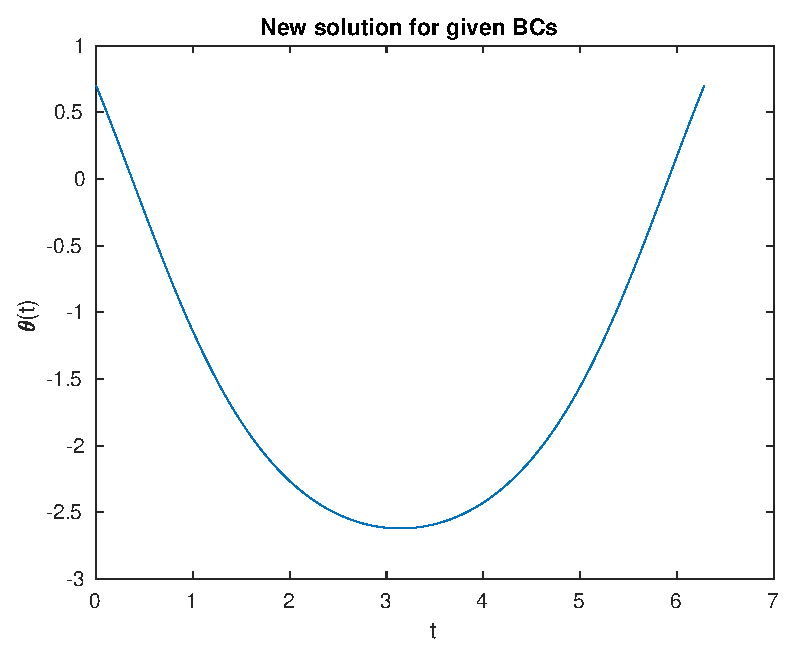
\includegraphics[scale=0.8]{hw3p1a.eps}\\

	\subsection{Part b}
To find a solution to this BVP with the same general behavior as figure 2.5 for a longer time interval, we choose our initial guess based on properties at our initial time interval $T=2\pi$. Namely, we reuse the computed solution for a smaller $T$ by using it as an initial guess (after scaling to the new time interval appropriately) for a larger time interval. The following plots display the solution that we obtain for $T=20,50,100,200$ by doing this recursively. \\
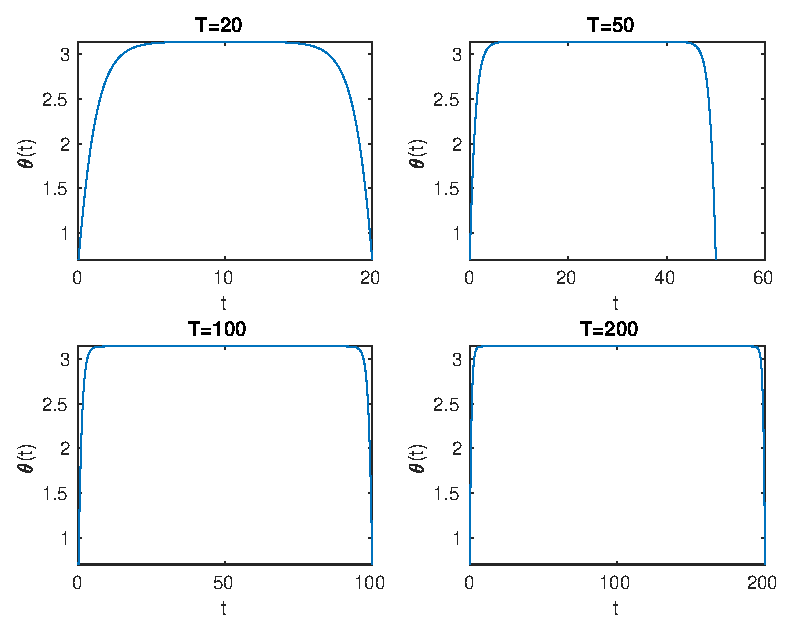
\includegraphics{hw3p1b.eps}\\
The following table lists the maximum value of $\theta$ obtained in each time interval. Clearly, they appear to be converging to $\pi$.
\begin{table}[H]\centering
\begin{tabular}{|r|r|}\hline
{T}&{$\max_i\theta_i$}\\\hline
$2\pi$&2.8975061095462498\\
20&      3.1413385828458429\\
50&      3.1415926535120287\\
100&      3.1415926535897931\\
200&     3.1415926535897931\\\hline
\end{tabular}
\end{table}
The following MATLAB code was used the obtain the results for this problem. 
\begin{verbatim}
T=2*pi;
m=2001;
t=linspace(0,T,m+2)';
h = t(2)-t(1);
alpha=0.7; beta=0.7;

theta=0.7+t.*(t-2*pi).^2;


theta = theta(2:end-1); %remove boundary
tol=1e-12; itermax=1000;
[theta,~,~]=NewtonSolve(theta,alpha,beta,h,tol,itermax);
figure(1)
plot(t,theta)
plot(t,theta)
xlabel('t'); ylabel('\theta(t)')
title('New solution for given BCs')
saveas(gcf,'hw3p1a','epsc')

i=1;
fprintf('T           max(theta)\n')

theta=0.7+sin(t/2);
theta = theta(2:end-1); %remove boundary
[theta,~,~]=NewtonSolve(theta,alpha,beta,h,tol,itermax);
fprintf('%i      %16.16d\n',T,max(theta))
figure(2)
for T=[20,50,100,200]
    t=linspace(0,T,m+2)';
    h = t(2)-t(1);
    theta = theta(2:end-1); %remove boundary, reuse old theta as new guess
    [theta,~,~]=NewtonSolve(theta,alpha,beta,h,tol,itermax);
    subplot(2,2,i)
    plot(t,theta)
    title(['T=',num2str(T)])
    xlabel('t')
    ylabel('\theta(t)')
    fprintf('%i      %16.16d\n',T,max(theta))
    i=i+1;   
end
saveas(gcf,'hw3p1b','epsc')

function G=buildG(theta,alpha,beta,h)

G=zeros(length(theta),1);
theta = [alpha; theta; beta]; %include BCs for computation 
for i=1:length(theta)-2
    G(i)=(theta(i)-2*theta(i+1)+theta(i+2))/h^2+sin(theta(i+1));
end

end


function J=buildJ(theta,h)

maindiag=-2+cos(theta)*h^2;
J=spdiags([ones(length(theta),1),maindiag,ones(length(theta),1)],-1:1,...
    length(theta),length(theta));
J=J/h^2;

end


function [theta,iter,dnormvec]=NewtonSolve(initial_guess,alpha,beta,h,tol,itermax)

theta = initial_guess;
deltanorm=Inf;
iter=0;
while deltanorm>tol && iter<itermax
    G=buildG(theta,alpha,beta,h);
    J=buildJ(theta,h);
    delta=-J\G;
    theta=theta+delta;
    deltanorm=norm(delta,'inf');
    iter=iter+1;
    dnormvec(iter)=deltanorm;
end

theta=[alpha;theta;beta]; %add BCs

end
\end{verbatim}
	
	\section{Problem 2}
	\subsection{Part a}
Consider the boundary value problem
\[
- u_{xx} + ( 1 + x^2 ) u = f ,~~0 \leq x \leq 1 ,
\]
\[
u(0) = 0 ,~~u(1) = 0
\]
on a uniform grid with spacing $h = 1/(m+1)$, with the following set of difference equations
that has local truncation error $O( h^2 )$:
\[
\frac{2 u_i - u_{i+1} - u_{i-1}}{h^2} + (1 + x_i^2 ) u_i = f( x_i ) ,~~i=1, \ldots , m .
\]
By Gerschgorin's theorem, we can sum the absolute values of the non-diagonal entries of the coefficient matrix $A$ associated with this set of difference equations to get that the Gerschgorin disks are given by
\[
B\left(\frac{2}{h^2}+1+x_1^2,\frac{1}{h^2}\right)=B\left(\frac{2}{h^2}+1+h^2,\frac{1}{h^2}\right)
\]
for $i=1$,
\[
B\left(\frac{2}{h^2}+1+x_m^2,\frac{1}{h^2}\right)=B\left(\frac{2}{h^2}+1+h^2m^2,\frac{1}{h^2}\right)
\]
for $i=m$, and
\[
B\left(\frac{2}{h^2}+1+x_i^2,\frac{2}{h^2}\right)=B\left(\frac{2}{h^2}+1+h^2i^2,\frac{2}{h^2}\right)
\]
for $i=2,\ldots,m-1$. We know that the eigenvalues of $A$ must be contained in the union of these disks, so observing that $A$ is symmetric so all eigenvalues are real, 
\begin{align*}
&\min_{i\in\{2,\ldots,m-1\}}\left\{\frac{1}{h^2}+1+h^2,\frac{1}{h^2}+1+h^2m^2,1+h^2i^2\right\}\leq\lambda\\&\leq\max_{i\in\{2,\ldots,m-1\}}\left\{\frac{3}{h^2}+1+h^2,\frac{3}{h^2}+1+h^2m^2,\frac{4}{h^2}+1+h^2i^2\right\}
\end{align*}
if $\lambda$ is an eigenvalue of $A$. Making the assumption that $m\geq1$ so that $0<h\leq\frac{1}{2}$, we can easily reduce this to 
\[
\min\left\{\frac{1}{h^2}+1+h^2,1+h^22^2\right\}\leq\lambda\leq\max\left\{\frac{3}{h^2}+1+h^2m^2,\frac{4}{h^2}+1+h^2(m-1)^2\right\}.
\]
Now, we note that with our restrictions on $m$ and $h$, $3h^4\leq3(1/2)^4=3/8<1$, so $1+4h^2<\frac{1}{h^2}+1+h^2$. Similarly, we can also conclude that $\frac{3}{h^2}+1+h^2m^2<\frac{4}{h^2}+1+h^2(m-1)^2$, so we can bound the eigenvalues of $A$ by
\[
1+4h^2\leq\lambda\leq\frac{4}{h^2}+1+h^2(m-1)^2.
\]
	\subsection{Part b}
To see that the $L_2$-norm of the global error is the same order as the local truncation error, we borrow the book's notation by letting $E$ be the global error and $\tau$ be the local truncation error and use the inequalities on page 19 to write
\[
\|E\|_{L_2}\leq\|A^{-1}\|_{L_2}\|\tau\|=\left(\min_i|\lambda_i|\right)^{-1}\|\tau\|\leq\|\tau\|=\OO(h^2).
\]
The reason for this is that we know that 1 is a lower bound on the eigenvalues of $A$, because the lower bound we found in part a is clearly greater than 1 when $h>0$.
	
\section{Problem 3}
Using the code from homework 2, we use the following to obtain approximate solutions at $h=.1$ and $h=.05$ compute a Richardson extrapolation 
\[
\phi_1(x_i;h)=\frac{4\Tilde{u}(x_i;h/2)-\Tilde{u}(x_i;h)}{3}
\]
in the standard way where $x_i$ denotes each gridpoint on the course grid.
\begin{verbatim}
m=9;
[u_coarse,h,errvec]=rodFD(c,utrue,ftrue,m);
errinf=norm(errvec,'inf');
fprintf('%.e       %.16e\n',h,errinf)

m=19;
[u_fine,h,errvec]=rodFD(c,utrue,ftrue,m);
errinf=norm(errvec,'inf');
fprintf('%.e       %.16e\n',h,errinf)

u_rich=(4*u_fine(1:2:end)-u_coarse)/3;
u_true=utrue(linspace(0,1,length(u_coarse)))';
errinf=norm(u_true-u_rich,'inf');
fprintf('Richardson       %.16e\n',errinf)
\end{verbatim}
The following table prints error results which appear to give higher order accuracy as one would expect.
\begin{table}[H]\centering
\begin{tabular}{|r|r|}\hline
{Approximation}&{Error in infinity norm}\\\hline
$\Tilde{u}(x;.1)$&2.1832687983814104e-03\\
$\Tilde{u}(x;.05)$&      5.4785209963363103e-04\\
$\varphi_1(x;.1)$&      2.7132000510379090e-06\\\hline
\end{tabular}
\end{table}
Now, if we instead assume that the coarse grid approximation is piecewise
linear, so that the approximation at the midpoint of each subinterval
is the average of the values at the two endpoints, one cannot use Richardson
extrapolation with the fine grid approximation and these interpolated
values on the coarse grid to obtain a more accurate approximation at
these points in general. While we can Taylor expand
\[
\frac{u(x+h)+u(x)}{2}-u(x+h/2)=\frac{hu'(x)+\OO(h^2)}{2}-(h/2)u'(x)+\OO(h^2)=\OO(h^2)
\]
to see that linear interpolation is also second order accurate, the issue lies in that we are using two different types of approximation. To see this more explicitly, say that the coefficient on the $h^2$ term in the error of our FD scheme is denoted $e(x)$ (with $x$ dependence to account for the fact that these terms typically include some derivative of $u$ evaluated at $x$), i.e. that 
\[
\Tilde{u}(x;h)=u(x)+e(x)h^2+\OO(h^3).
\]
Then, for our fine grid,
\[
\Tilde{u}(x;h/2)=u(x)+e(x)\frac{h^2}{4}+\OO(h^3).
\]
However, for the interpolation on our coarse grid, the approximation at a midpoint $x$ is 
\begin{align*}
\frac{\Tilde{u}(x+h/2;h)+\Tilde{u}(x-h/2;h)}{2}&=\frac{u(x+h/2)+e(x+h/2)h^2+u(x-h/2)+e(x-h/2)h^2+\OO(h^3)}{2}\\&=
\frac{u(x+h/2)+u(x-h/2)}{2}+\frac{e(x+h/2)h^2+e(x-h/2)h^2}{2}+\OO(h^3)\\&=
u(x)+\frac{h^2}{4}u''(x)+\frac{e(x+h/2)h^2+e(x-h/2)h^2}{2}+\OO(h^3)\\&=
u(x)+\frac{h^2}{4}u''(x)+\frac{h^2}{2}(2e(x)+\OO(h^2))+\OO(h^3)\\&=
u(x)+(u''(x)/4+e(x))h^2+\OO(h^3)
\end{align*}
if we assume that $e$ permits a Taylor expansion at $x$. In order for our standard Richardson extrapolation technique to work, we need to be able to eliminate the $h^2$ term by scaling the approximation on the fine grid by $2^2=4$. However, this will only work here if $e(x)=u''(x)/4+e(x)$, i.e. that $u''(x)=0$ which is not necessarily true in general. It would be difficult to even modify Richardson extrapolation to work here since $u''(x)$ is not necessarily known.
%Thus, the only way to eliminate the $h^2$ term between our 2 approximations is for $e(x)$ to be some scalar multiple of $u''(x)+2e(x+h/2)+2e(x-h/2)$, so this does not work for the general case. 

\section{Problem 4}
Differentiating the nonlinear difference equations (2.106) to get a Jacobian, we can see that 
\[
J_{i,j}=\begin{cases}
-\frac{2\epsilon}{h^2}+\frac{u_{i+1}-u_{i-1}}{2h}-1, \quad &j=i\\
\frac{\epsilon}{h^2}+\frac{u_i}{2h}, \quad &j=i+1\\
\frac{\epsilon}{h^2}-\frac{u_i}{2h}, \quad &j=i-1\\
0, \quad &\text{otherwise},
\end{cases}
\]
for $i,j=1,\ldots m$ noting that $u_0=\alpha$, $u_{m+1}=\beta$. With this, we apply Newton's method to solve (2.106) on the standard grid $a=x_0<x_1<\ldots<x_m<x_{m+1}=b$ with the standard spacing $h=x_{i+1}-x_i$ for $a=0$, $b=1$, $\alpha = -1$, $\beta = 1.5$, and $\epsilon = 0.01$. We do so for $h=1/20$, $h=1/40$, $h=1/80$, and $h=1/160$ and plot the results on top of each other as follows.\\
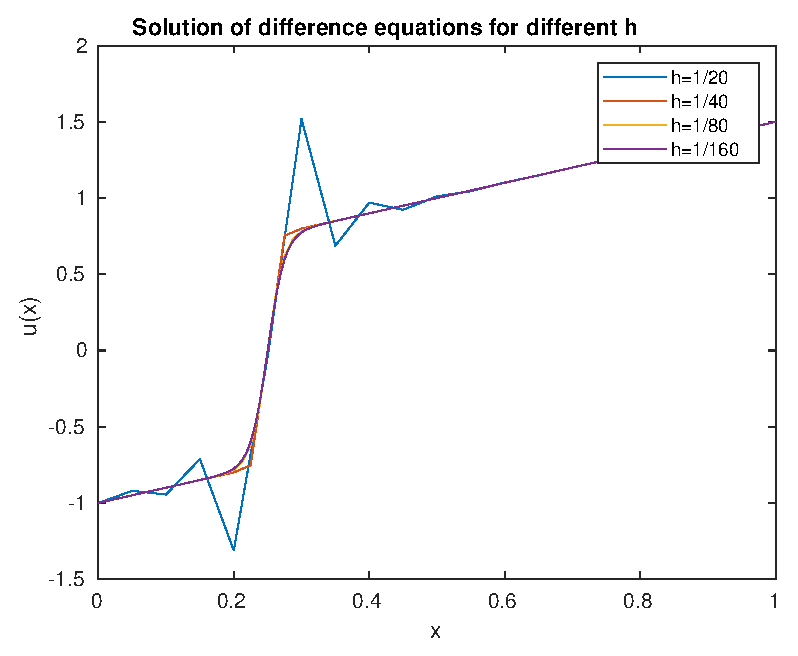
\includegraphics[scale=0.8]{hw3p4.eps}\\
The following MATLAB code was used to solve the equations and create the above plot. Newton's method is used with a stopping tolerance of $\|\delta^{[k]}\|_\infty<10^{-12}$ and an initial guess of the function defined in (2.105) with the values of $w_0$ and $\Bar{x}$ as given in (2.103) and (2.104), respectively is built in the function "buildinitialguess."
\begin{verbatim}
figure(1)
for m=[19 39 79 159] 
    a=0; b=1; alpha=-1; beta=1.5; epsilon=0.01;
    x=linspace(a,b,m+2)';
    h = x(2)-x(1);
    tol=1e-12; itermax=100;

    initial_guess=buildinitialguess(x(2:end-1),a,b,alpha,beta,epsilon);
    [u,iter,dnormvec]=NewtonSolve(initial_guess,alpha,beta,epsilon,h,tol,itermax);
    plot(x,u)
    hold on
end
xlabel('x')
ylabel('u(x)')
legend('h=1/20','h=1/40','h=1/80','h=1/160')
title('Solution of difference equations for different h')
hold off
saveas(gcf,'hw3p4','epsc')

function u=buildinitialguess(x,a,b,alpha,beta,epsilon) %function from 2.105

w0=(a-b+beta-alpha)/2;
xbar=(a+b-alpha-beta)/2;
u=x-xbar+w0*tanh(w0*(x-xbar)/(2*epsilon));

end



function G=buildG(u,alpha,beta,h,epsilon)

G=zeros(length(u),1);
u = [alpha; u; beta];
for i=1:length(u)-2
    G(i)=epsilon*(u(i)-2*u(i+1)+u(i+2))/h^2+u(i+1)*((u(i+2)-u(i))/(2*h)-1);
end

end



function J=buildJ(u,alpha,beta,h,epsilon)

u = [alpha; u; beta];

for i=1:length(u)-2
    Jdiag(i)=-2*epsilon/h^2+(u(i+2)-u(i))/(2*h)-1;
end
Jsuperdiag=epsilon/h^2+u(1:end-2)/(2*h);
Jsubdiag=epsilon/h^2-u(3:end)/(2*h);

J=spdiags([Jsubdiag,Jdiag',Jsuperdiag],-1:1,length(u)-2,length(u)-2);

end


function [u,iter,dnormvec]=NewtonSolve(initial_guess,alpha,beta,epsilon,h,tol,itermax)

u = initial_guess;
deltanorm=Inf;
iter=0;
while deltanorm>tol && iter<itermax
    G=buildG(u,alpha,beta,h,epsilon);
    J=buildJ(u,alpha,beta,h,epsilon);
    delta=-J\G;
    u=u+delta;
    deltanorm=norm(delta,'inf');
    iter=iter+1;
    dnormvec(iter)=deltanorm;
end

u=[alpha;u;beta]; %add BCs

end
\end{verbatim}

\end{document}